\documentclass{sig-alternate-05-2015}
%\usepackage[margin=.7in]{geometry} 
\usepackage{amsmath,amssymb}
\usepackage{mathpartir}
\usepackage{scrextend}
\usepackage{hyperref}
\usepackage{algorithm}
\usepackage{algpseudocode}
\usepackage{color}
\usepackage{listings}

\definecolor{mygreen}{rgb}{0,0.6,0}
\definecolor{mygray}{rgb}{0.5,0.5,0.5}
\definecolor{mymauve}{rgb}{0.58,0,0.82}

\lstset{
basicstyle=\tiny,
breaklines=true,
language=Java,
%backgroundcolor=\color{white},
captionpos=b,
commentstyle=\color{mygreen},
%frame=single,
keywordstyle=\color{blue},
numberstyle=\color{mygray},
stringstyle=\color{mymauve},
}

\begin{document}
\setcopyright{none}

\title{Multiclass Logistic Regression using Harp}
\numberofauthors{2}
\author{
  \alignauthor Chao-Hong Chen\\
  \affaddr{Indiana University}\\
  \email{chen464@indiana.edu}
  \alignauthor Qiuwei Shou\\
  \affaddr{Indiana University}\\
  \email{qiuwshou@umail.iu.edu}
}
\makeatletter
\def\@copyrightspace{\relax}
\makeatother
\maketitle

\section{Introduction}
MLR (Multiclass Logistic Regression) is a very common problem in machine learning,
and in practice we usually need to deal with very huge data sets so exploit parallelism
to achieve speed up is important.\par
In this project, we will try to apply Harp\cite{harp} on MLR.
The algorithm we use will be based on is Stochastic Gradient descent (SGD).
The reference implementations are \cite{logistic-regression} and scikit-learn\cite{scikit-learn} which is a python library,
we will try to use Harp to parallelize the algorithm to handle large datasets.\par
In section \ref{sec:prob}, we will beiefly describe the MLR problems and SGD,
in section \ref{sec:method} we will describe our Harp version of SGD for MLR,
in section \ref{sec:eval} we will evaluate our algorithm using RCV1v2\cite{Lewis:2004:RNB:1005332.1005345}
and we conclude this project in section \ref{sec:con}.

\section{Problem description}\label{sec:prob}
The logistic regression is a classification method used to predict binary class labels with given a set $n$ variables.
So what we want is for given input $x_1, \ldots, x_n$ and a class $C$,
\begin{align}
  h(x_1,\ldots,x_n) =
  \begin{cases}
    1 , & (x_1,\ldots,x_n) \in C \\
    0 , & \text{otherwise.}
  \end{cases}
\end{align}
In this project we will use linear model:
\begin{align}
  f(\overline{x}) = \theta_0 + \sum_{i=1}^n x_i \cdot\theta_i =
  \begin{pmatrix} 1 \; x_1 \; \ldots \; x_n \end{pmatrix} \cdot
  \begin{pmatrix}\theta_0\\\theta_1\\ \vdots \\ \theta_n\end{pmatrix}
\end{align}
We will denote $\overline{x} = \begin{pmatrix} 1 \; x_1 \; \ldots \; x_n \end{pmatrix}$ and $\overline{\theta} = \begin{pmatrix}\theta_0 \; \theta_1 \;\ldots \; \theta_n\end{pmatrix}$ in the rest of this article.\\
Given $\overline{\theta}$ we can use the sigmoid function to define our predictor:
\begin{align}\label{eq:1}
h_{\overline{\theta}}(\overline{x}) = \frac{1}{1+e^{- f(\overline{x})}} = \frac{1}{1+e^{- \overline{x} \cdot\overline{\theta}^T}}
\end{align}
A set of training samples containts $\overline{x_1}, \ldots \overline{x_m}$ and the classified label
$y_i =   
\begin{cases}
  1 , & \overline{x_i} \in C \\
  0 , & \text{otherwise.}
\end{cases}$,
for a set of training samples we can define the cost function $J(\overline{\theta})$ as:
\begin{align}\label{eq:2}
J(\overline{\theta}) = - \frac{1}{m} \sum_{i=1}^m y_i \log h_{\overline{\theta}} (\overline{x_i})+(1-y_i)\log(1-h_{\overline{\theta}} (\overline{x_i}))
\end{align}
It is obvious that if $J(\overline{\theta}) = 0$ then our predictor $h_{\overline{\theta}}(\overline{x})$ correctly predict every sample in the training set,
so our goal is to find $\overline{\theta}$ to minimize $J(\overline{\theta})$.\\
There are multiple ways to update the parameter for minimizing the cost function,
in this project we choose Stochastic Gradient descent (SGD).
In SGD the $\overline{\theta}$ will be initialize randomly and then SGD will randomly choose a training sample $\overline{x_i}$ and update the parameters $\overline{\theta}$ with given learning rate $\alpha$ by calculating the partial derivatives:
\begin {align} \label{eq:3}
\overline{\theta} := \overline{\theta} - \alpha \frac{1}{m} \sum_{i=1}^m (h_{\overline{\theta}} (\overline{x_i}) - y_i) \cdot \overline{x_i}
\end{align}
$\overline{\theta}$ will be updated for given amount of iterations or until converge.\par
The MLR generalizes the logistic regression by applying it to multi-class classification.
So instead of just single class $C$, in MLR we have $C_1, \ldots, C_k$ class and any $\overline{x}$
can belongs to multiple classes.
We can still use SGD to solve MLR by running SGD seperately for each class.
\section{Proposed Method}\label{sec:method}
We made some modification to SGD, instead of randomly choose a sample we choose it in order to guarantee deterministic result.
So given the number of iterations $ITER$ the SGD becomes:
\begin{algorithm}
  \begin{algorithmic}[1]
    \State initialize $\overline{\theta}$
    \For{$j = 1$ to $ITER$}
    \For{$i=1$ to $m$}
    \State $\overline{\theta} := \overline{\theta} - \alpha \frac{1}{m} \sum_{i=1}^m (h_{\overline{\theta}} (\overline{x_i}) - y_i) \cdot \overline{x_i}$
    \EndFor
    \EndFor
  \end{algorithmic}
\end{algorithm}\\
Note, this can be easily modified to the original SGD by choosing $i$ randomly for $m$ times.\par

The whole flow of harpMLR is given in  \ref{fig:sketch}.
\begin{figure}
  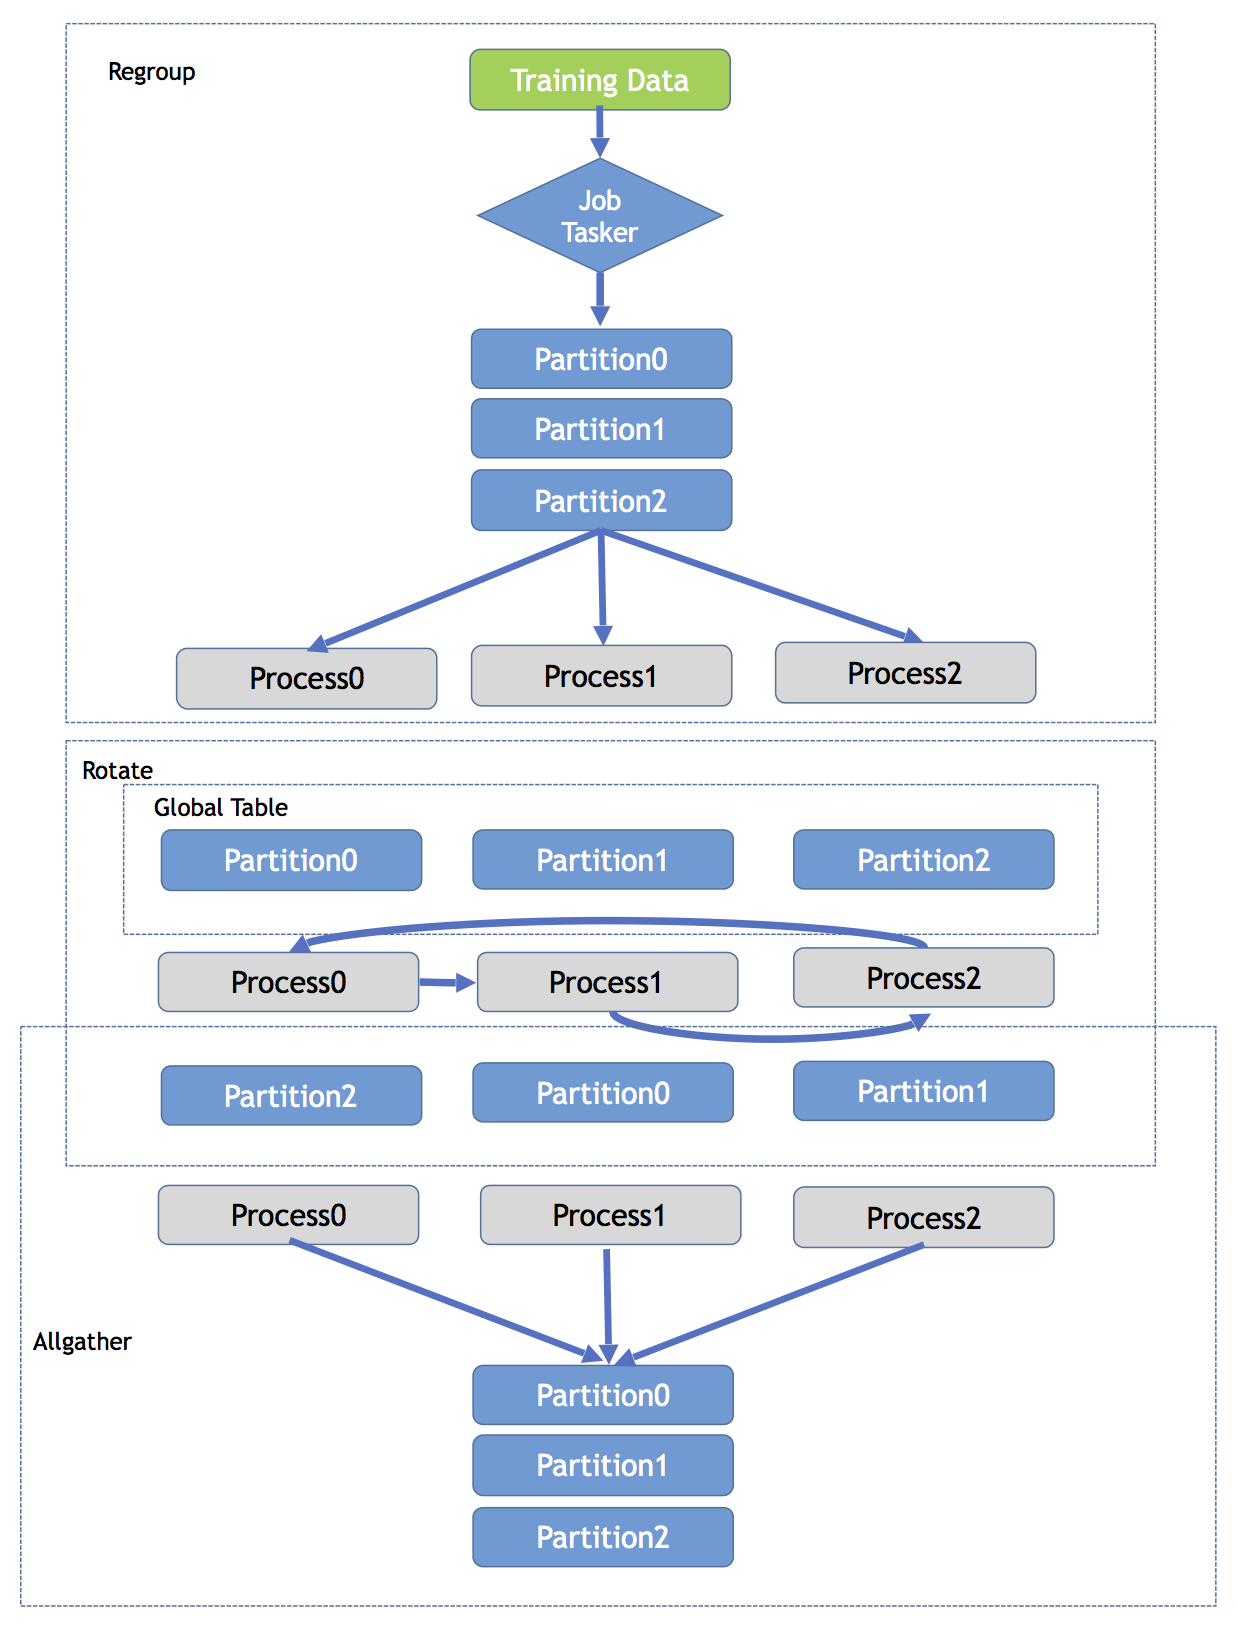
\includegraphics[scale=0.45]{fig/sketch.png}
  \caption{The whole flow of harpMLR}
  \label{fig:sketch}
\end{figure}

In our parallel SGD, we distribute the training data across each mapper,
each mapper loads assigned part of the dataset at first, see figure \ref{fig:load}.
\begin{figure}
\begin{lstlisting}
private void LoadAll(KeyValReader reader) throws IOException, InterruptedException {
  topics = Util.LoadTopicList(topicPath, conf);
  qrels = Util.LoadQrels(qrelsPath, conf);
  data = new ArrayList<Instance>();

  while (reader.nextKeyValue()) {
    String value = reader.getCurrentValue();
    Util.LoadData(value, conf, data);
  }
}
\end{lstlisting}
\caption{Load trainging data}
\label{fig:load}
\end{figure}

\begin{figure}
\begin{lstlisting}
private Table<DoubleArray> wTable;
  
private void initTable() {
  wTable = new Table(0, new DoubleArrPlus());
  for (int i = 0; i < topics.size(); ++i) {
    wTable.addPartition(new Partition(i, DoubleArray.create(TERM + 1, false)));
  }
}
\end{lstlisting}
\caption{Create tables}
\label{fig:init}
\end{figure}

Then we create a table which contain $\overline{\theta}$ for each class (see figure \ref{fig:init}),
and initialize the scheduler which will manage threads that perform SGD (see figure \ref{fig:thread}).\par

\begin{figure}
\begin{lstlisting}
private List<GDtask> GDthread;
private DynamicScheduler<Partition, Object, GDtask> GDsch;

private void initThread() {
  GDthread = new LinkedList<>();
  for (int i = 0; i < numThread; i++) {
    GDthread.add(new GDtask(alpha, data, topics, qrels));
  }
  GDsch = new DynamicScheduler<>(GDthread);
}
\end{lstlisting}
\caption{Initialize scheduler}
\label{fig:thread}
\end{figure}


Next we distribute all $\overline{\theta}$s across map use \lstinline|regroup| provided by Harp,
after this each mapper get a set of class $C_{i_1},\ldots,C_{i_n}$ and the corresponding $\overline{\theta_{i_j}}$.
For each iteration, every mapper submit job to thread scheduler to compute SGD for every the given set of class,
the scheduler will assign thread to compute SGD using the training data the mapper have loaded,
and update each $\overline{\theta_{i_j}}$ (see figure \ref{fig:GD}), we use \lstinline|ratate| to passing the updated $\overline{\theta}$s to other mapper and
receiving another set of class and corresponding $\overline{\theta}$s from other thread.
Repeat this for number of mapper times is equal to update all $\overline{\theta}$s for the whole training data set (see figure \ref{fig:SGD}).
After the given number of iterations, we use \lstinline|allgather| to collect all $\overline{\theta}$s and output the final $\overline{\theta}$s.

\begin{figure}
  \begin{lstlisting}
public class GDtask implements Task<Partition, Object> {
  private double alpha;
  private HashMap<Integer, ArrayList<String>> qrels;
  private ArrayList<Instance> data;
  private ArrayList<String> topics;

  public GDtask(double A, ArrayList<Instance> D, ArrayList<String> T,
                HashMap<Integer, ArrayList<String>> Q) {
    qrels = Q;
    alpha = A;
    data = D;
    topics = T;
  }

  @Override
  public Object run(Partition par) throws Exception {
    String cat = topics.get(par.id());
    double[] W = ((DoubleArray)par.get()).get();
    double p;
    double label;
    Instance inst;

    for (int i = 0; i < data.size(); ++i) {
      inst = data.get(i);
      p = predict(W, inst.term);
      if (qrels.get(inst.id).contains(cat))
        label = 1.0;
      else
        label = 0.0;

      W[0] += alpha * (label - p); // constant
      for(Map.Entry<Integer, Double> entry : inst.term.entrySet()) {
        int key = entry.getKey();
        double value = entry.getValue();

        W[key] += alpha * (label - p) * value;
      }
    }
    return null;
  }

  private static double sigmoid(double z) {
    return 1.0 / (1.0 + Math.exp(-z));
  }

  private static double predict(double W[], HashMap<Integer, Double> x) {
    double res = W[0]; // constant

    for(Map.Entry<Integer, Double> entry : x.entrySet()) {
      int key = entry.getKey();
      double value = entry.getValue();

      res += W[key] * value;
    }
    
    return sigmoid(res);
  }
}
\end{lstlisting}
\caption{Gradient decent task}
\label{fig:GD}
\end{figure}

%Harp provides different collective communication models. It's able to use regroup and allgather to achieve the implementation of allreduce from MPI collective communication. Regroup defines the name of operations and broadcast the data structure of regrouping data. It also sends the partitioned data to corresponding processes. Inside each iteration, the partial MLR model will be individually trained by computing GD with the partitioned data in its own process. Calling the rotate the model will rotate through the processes and keep updating the each MLR model parameters to make sure the model is consistent. In the end, all computed results will be collected by allgather. The implementation of parallelized GD on harp is shown below: 
\begin{figure}
\begin{lstlisting}[language=java]
protected void mapCollective(KeyValReader reader, Context context) throws IOException, InterruptedException {
  LoadAll(reader);
  initTable();
  initThread();
  regroup("MLR", "regroup_wTable",wTable,
          new Partitioner(getNumWorkers()));

  GDsch.start();        
  for (int iter = 0; iter < ITER * numMapTask; ++iter) {
    // submit job
    for (Partition par : wTable.getPartitions()) {
      GDsch.submit(par);
    }
    // wait until all job completed
    while (GDsch.hasOutput()) {
      GDsch.waitForOutput();
    }
            
    rotate("MLR", "rotate_" + iter, wTable, null);

    context.progress();
  }
  GDsch.stop();
  allgather("MLR", "allgather_wTable", wTable);

  if (isMaster()) {
    Util.outputData(outputPath, topics, wTable, conf);
  }

  wTable.release();
}
\end{lstlisting}
\caption{Harp SGD}
\label{fig:SGD}
\end{figure}
\section{Evaluation}\label{sec:eval}
In this section we will conducting evaluation of our algorithm using RCV1v2\cite{Lewis:2004:RNB:1005332.1005345}.
RCV1v2 is a text categorization test collection, we will use our algorithm to classify the topic of documents.
There are 103 topics in RCV1v2, and for each document there are 47236 terms.
So we have 103 classes, and every instance is a $47237$ dimension vector (add 1 for constant).
The original training set in \cite{Lewis:2004:RNB:1005332.1005345} contains 23149 training vector which is very small,
since the point of this evaluation is to test the capibility of our algorithm to handle large data set,
so we use the original test data as our training data which contains 781265 vectors.\par
We use two machines each has Intel(R) Xeon(R) CPU E5-2670 v3 with 128GB ram.
Figure \ref{fig:runtime} shows the runtime of our algorithm with 2 and 4 mappers for 100 iterations with 1 to 16 local thread,
figure \ref{fig:speedup} shows the speedup with different number of local thread.
\begin{figure}
  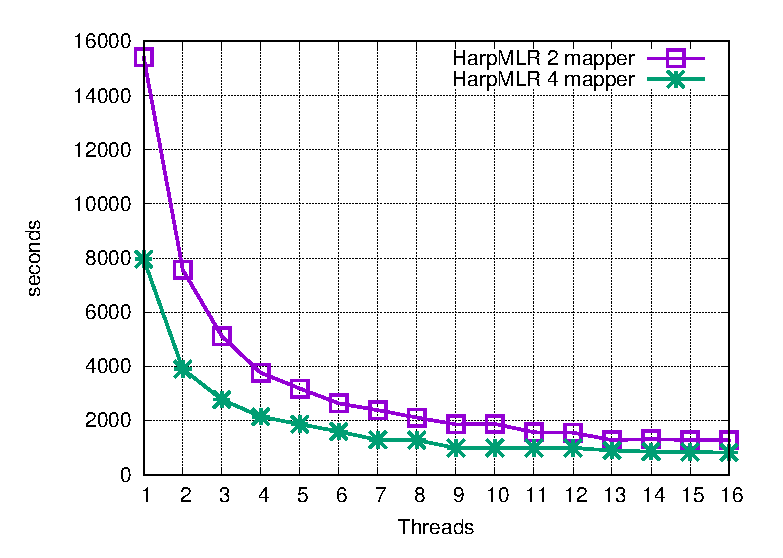
\includegraphics[scale=0.7]{fig/runtime.eps}
  \caption{Runtime of HarpMLR with 2 mappers}
  \label{fig:runtime}
\end{figure}

\begin{figure}
  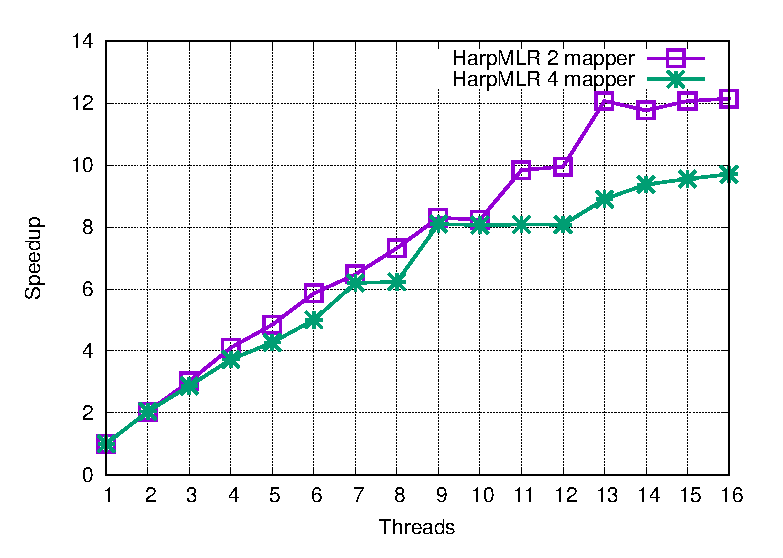
\includegraphics[scale=0.7]{fig/speedup.eps}
  \caption{Speedup of HarpMLR with 2 mappers}
  \label{fig:speedup}
\end{figure}
According to the results, increase local thread number gives almost linear speedup,
and increase local thread number is slightly faster than increase number of mappers.\par
We also use the training set in \cite{Lewis:2004:RNB:1005332.1005345} to caculate the effectiveness of the output results,
the macroaveraged $F_{1.0}$ (defined in \cite{Lewis:1995:EOA:215206.215366}) is $0.62$.
Note since the training data we use is a lot larger than the test data,
the purpose of this is not mean to show that our algorithm is very effective,
but merely to verify that the output of our algorithm is what we expected.

\section{Conclusion}\label{sec:con}
In this project we propose a parallel version of SGD to solve MLR using Harp,
and we evaluate our algorithm using RCV1v2.
According to the results, we achive expected speedup from increase number of mappers and increase number of local threads.

\bibliographystyle{abbrv}
\bibliography{bib/refs}

\clearpage
\noindent
Job assignment:\\
Chao-Hong Chen:
\begin{enumerate}
\item implement harpMLR, sequential MLR
\item running experiments
\item writing report
\end{enumerate}
Qiuwei Shou:
\begin{enumerate}
\item set up hadoop and harp
\item implement code proceess RCV1v2 (Util.java)
\item writing report
\item poster
\end{enumerate}

\end{document}
